% KaushalDub -- IEEE conference paper (IEEEtran, two columns, max. 6 pages).
% Compile on Overleaf with pdfLaTeX (upload this file + figures/). All numbers come from
% docs/paper/metrics.json, produced by docs/paper/compute_metrics.py from the project's own outputs.
\documentclass[conference]{IEEEtran}
\IEEEoverridecommandlockouts
\usepackage{cite}
\usepackage{amsmath,amssymb}
\usepackage{graphicx}
\usepackage{booktabs}
\usepackage{multirow}
\usepackage{xcolor}
\usepackage{tikz}
\usetikzlibrary{arrows.meta,positioning,fit,calc}
\usepackage[hidelinks]{hyperref}
\definecolor{kdteal}{HTML}{0B6E6E}
\definecolor{kdamber}{HTML}{D9822B}
\newcommand{\rup}{Rs.\,}

\begin{document}

\title{KaushalDub: Step-Aligned Hindi and Kannada Dubbing of Vocational How-To Videos using Temporal Action Segmentation and Indic Speech Models}

% Fill in the remaining team members and the guide in the same format.
\author{
\IEEEauthorblockN{Nitish Patil}
\IEEEauthorblockA{B.Tech (H), 3rd year\\
RV University\\
Bengaluru, India\\
nitishpatil.btech23@rvu.edu.in}
\and
\IEEEauthorblockN{[Co-author name]}
\IEEEauthorblockA{B.Tech (H), 3rd year\\
RV University\\
Bengaluru, India\\
[email]@rvu.edu.in}
\and
\IEEEauthorblockN{[Guide name]}
\IEEEauthorblockA{[Department]\\
[Institution]\\
Bengaluru, India\\
[email]}
}

\maketitle

\begin{abstract}
Short demonstration videos are a common way to teach vocational skills, but most of them are narrated in English, which
limits their reach among learners who work in Hindi or Kannada. We present KaushalDub, a system that segments a how-to
video into its procedural steps, writes a short grounded instruction for each step, and produces a dubbed version in Hindi
and Kannada with captions and a quiz. The core of the system is a step recogniser that combines frozen CLIP ViT-B/16
frame features with a two-stage temporal convolutional network and cosine classification heads initialised from CLIP
text embeddings. On three target skills from the COIN dataset, we compare it against a ResNet-50 + BiLSTM baseline, an
X-CLIP video encoder with a linear head, a CLIP + BiLSTM ablation and CLIP zero-shot classification. The proposed model
reaches a macro-F1 of 42.3 and an F1@50 of 34.3, close to the best ablation (44.3) while using one third of its trainable
parameters, training five times faster and giving the lowest uncalibrated expected calibration error (3.9\%). We also
compare commercial and open Indic speech stacks stage by stage and report the measured cost of dubbing a 30-video
library: \rup4.07 and 4.6 minutes per video on average. A human-in-the-loop correction memory lets annotator
corrections improve later videos of the same skill without retraining.
\end{abstract}

\begin{IEEEkeywords}
temporal action segmentation, instructional video, CLIP, MS-TCN, automatic dubbing, Indic languages, text-to-speech,
active learning
\end{IEEEkeywords}

\section{Introduction}
Vocational training in India increasingly relies on short demonstration videos: how to perform CPR, fit a screen
protector or polish a car. Most freely available tutorials are narrated in English, while many trainees are more
comfortable in a regional language. Re-recording each video for every language is slow and costly, and plain machine
translation of the soundtrack does not help when the instructor says little or the audio is only music.

A procedural video has structure that a dubbing system can exploit. The steps occur in a fixed order, each step occupies
a time interval, and a learner mainly needs to know what to do during each interval. KaushalDub therefore first detects
the steps visually and then narrates them, rather than translating the audio word for word. This makes the dub
independent of whether the original has speech, keeps the narration aligned with the action on screen, and gives the
trainer a small, reviewable set of sentences instead of a full transcript.

Existing work treats the pieces separately. Temporal action segmentation models such as MS-TCN~\cite{farha2019mstcn} and
ASFormer~\cite{yi2021asformer} label frames of instructional videos~\cite{tang2019coin,zhukov2019crosstask}, while
automatic dubbing research focuses on aligning translated speech with the original utterances~\cite{federico2020dubbing,
oktem2019prosodic}. Indian-language models for translation~\cite{gala2023indictrans2}, speech
recognition~\cite{bhogale2023vistaar} and speech synthesis~\cite{lyth2024parler} have matured, but they are rarely
evaluated together on an end-to-end task with real cost constraints. The contributions of this paper are:
\begin{itemize}
\item a systematic comparison of five step-recognition architectures on the same COIN splits, covering accuracy, step
order, boundaries, calibration, parameters and training time;
\item a step-aligned dubbing pipeline that grounds LLM-written narration in the detected steps and the transcript and
places synthesised speech with a bounded speed-up;
\item a stage-by-stage comparison of a commercial Indic API (Sarvam) and open AI4Bharat models, and measured cost and
latency for a 30-video, four-domain library;
\item a correction memory that blends annotator-approved segments into the class prototypes, with a retraining rule that
only accepts a new model if its test macro-F1 is not lower.
\end{itemize}

\section{Related Work}
\textbf{Temporal action segmentation.} Lea et al.~\cite{lea2017tcn} introduced temporal convolutional networks for
action segmentation together with the segmental F1@$k$ and edit metrics. MS-TCN~\cite{farha2019mstcn} stacks
dilated residual stages that refine each other's predictions and adds a truncated smoothing loss against
over-segmentation; ASFormer~\cite{yi2021asformer} replaces convolutions with attention. Most of these methods use I3D
features; we instead evaluate image--text pre-trained features~\cite{radford2021clip}, which also allow class vectors to
be initialised from step names. COIN~\cite{tang2019coin} and CrossTask~\cite{zhukov2019crosstask} provide step
annotations for instructional videos, and HowTo100M~\cite{miech2019howto100m} showed that narrated tutorials are a rich
source of weak supervision.

\textbf{Video encoders.} Besides frame-level CNN features~\cite{he2016resnet} followed by recurrent models~\cite{hochreiter1997lstm},
video-specific encoders such as X-CLIP~\cite{ni2022xclip} extend CLIP with cross-frame attention. We compare both
families under identical downstream training.

\textbf{Dubbing and Indic speech.} Automatic dubbing systems translate and re-synthesise speech while respecting the
timing of the original~\cite{federico2020dubbing,oktem2019prosodic}. For Indian languages, IndicTrans2~\cite{gala2023indictrans2}
covers all 22 scheduled languages, AI4Bharat's Vistaar benchmarks~\cite{bhogale2023vistaar} track ASR progress, and
Parler-TTS~\cite{lyth2024parler} enables controllable synthesis. Whisper~\cite{radford2023whisper} provides multilingual
recognition with language identification. Our work differs in that the visual step structure, not the speech, defines
the dubbing timeline.

\section{Proposed System}
Fig.~\ref{fig:arch} shows the pipeline. Stages 1--4 run after upload and produce reviewable step text; stages 5--7 run
after the trainer approves.

\begin{figure*}[t]
\centering
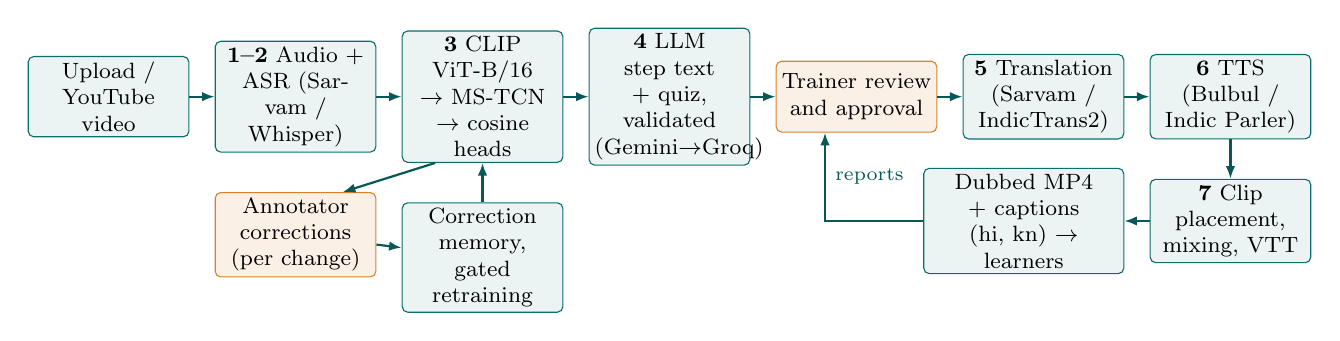
\begin{tikzpicture}[font=\footnotesize, node distance=3.2mm,
  box/.style={draw=kdteal, fill=kdteal!8, rounded corners=2pt, align=center, minimum height=9mm, text width=19mm, inner sep=2pt},
  hum/.style={box, draw=kdamber, fill=kdamber!12},
  arr/.style={-{Latex[length=1.6mm]}, thick, kdteal!80!black}]
\node[box] (vid) {Upload / YouTube\\video};
\node[box, right=of vid] (asr) {\textbf{1--2} Audio +\\ASR (Sarvam /\\Whisper)};
\node[box, right=of asr] (step) {\textbf{3} CLIP ViT-B/16\\$\rightarrow$ MS-TCN\\$\rightarrow$ cosine heads};
\node[box, right=of step] (llm) {\textbf{4} LLM step text\\+ quiz, validated\\(Gemini$\rightarrow$Groq)};
\node[hum, right=of llm] (rev) {Trainer review\\and approval};
\node[box, right=of rev] (mt) {\textbf{5} Translation\\(Sarvam /\\IndicTrans2)};
\node[box, right=of mt] (tts) {\textbf{6} TTS (Bulbul /\\Indic Parler)};
\node[box, below=5mm of tts] (mix) {\textbf{7} Clip placement,\\mixing, VTT};
\node[box, left=of mix, text width=24mm] (out) {Dubbed MP4 + captions\\(hi, kn) $\rightarrow$ learners};
\node[hum, below=5mm of asr] (ann) {Annotator\\corrections\\(per change)};
\node[box, below=5mm of step] (mem) {Correction\\memory, gated\\retraining};
\draw[arr] (vid) -- (asr); \draw[arr] (asr) -- (step); \draw[arr] (step) -- (llm); \draw[arr] (llm) -- (rev);
\draw[arr] (rev) -- (mt); \draw[arr] (mt) -- (tts); \draw[arr] (tts) -- (mix); \draw[arr] (mix) -- (out);
\draw[arr] (out.west) -| ([xshift=-4mm]rev.south) node[pos=0.75, right, font=\scriptsize] {reports};
\draw[arr] ([xshift=-6mm]step.south) -- ([xshift=6mm]ann.north); \draw[arr] (ann) -- (mem);
\draw[arr] (mem.north) -- (step.south);
\end{tikzpicture}
\caption{KaushalDub architecture. Teal: automatic stages; amber: human-in-the-loop. Every provider stage has a
fallback order, and a stage pauses with a ``needs credits'' state when no provider is left.}
\label{fig:arch}
\end{figure*}

\subsection{Step recogniser}
Frames are sampled at 2\,fps (at most 900 frames) and centre-cropped to $224\times224$. A frozen encoder maps each frame
to a feature $x_t$. The main model, \emph{CLIP + MS-TCN}, uses the 512-d image embedding of CLIP ViT-B/16 and two
temporal stages, each with six dilated residual layers (128 channels, dilation $2^i$). Each stage $s$ projects its
hidden state to an embedding $z^{(s)}_t = \mathrm{norm}(P_s h^{(s)}_t + x_t)$; the projection is zero-initialised, so the
model starts from the raw CLIP feature. Logits are scaled cosine similarities with one weight matrix $W^{(k)}$ per skill
$k$:
\begin{equation}
\ell_{t,c} = \gamma \, \frac{z_t^\top w^{(k)}_c}{\lVert w^{(k)}_c\rVert}, \qquad \gamma = e^{\theta},
\end{equation}
where $w^{(k)}_c$ is initialised with the mean CLIP text embedding of the step name under three prompt templates
(``a person who is about to \ldots'') and $\theta$ is learned. This initialisation makes the untrained model a CLIP
zero-shot classifier and makes new skills addable as prototypes. Training minimises, over both stages,
\begin{equation}
\mathcal{L} = \sum_{s}\Big[\mathrm{CE}_{\omega}\big(\ell^{(s)}, y\big) + \lambda \,\tfrac{1}{T}\sum_{t}\min\big(\Delta_{t}^{2}, 16\big)\Big],
\end{equation}
with class weights $\omega_c \propto n_c^{-1/2}$, $\lambda = 0.15$ and $\Delta_t$ the change in log-probabilities between
consecutive frames, as in MS-TCN~\cite{farha2019mstcn}. A per-skill temperature fitted on the validation set calibrates
the softmax~\cite{guo2017calibration}. At inference, segments shorter than 2\,s take the label of their longer
neighbour, adjacent segments with the same label are joined, and steps with mean confidence below 0.6 are flagged as
low-confidence; their keyframes are passed to the LLM.

\subsection{Grounded step text}
For each detected step the LLM receives its time span, label, confidence, the transcript inside the span and a word
budget of two words per second. The prompt forbids adding facts that are not in the speech or the label. The response
must contain exactly one entry per step in the original order; it is validated, retried once, and replaced by a
label-based template if it still fails. Providers are tried in order (Gemini~\cite{gemini2023}, a second Gemini model
when the first is overloaded, then an open-weight model served by Groq, GPT-OSS-120B in our runs), and small format slips are repaired before validation.

\subsection{Translation, speech synthesis and timing}
Narration lines are translated into Hindi and Kannada and synthesised per step. Clip $i$ of duration $d_i$ starts at
$a_i = \max(s_i, b_{i-1}+0.15)$, where $s_i$ is the step start and $b_{i-1}$ the end of the previous clip. If it does not
fit before the next step starts at $s_{i+1}$, it is sped up by
\begin{equation}
\rho_i = \min\!\big(1.3,\; d_i/(s_{i+1}-a_i)\big),
\end{equation}
and any remainder pushes the next clip later, so the order of steps is never changed. The narration is mixed over the
original soundtrack at 15\% volume, and WebVTT captions are written from the final placements. A second mode translates
every transcript sentence instead of the step narration and lowers the original track to 5\%.

\subsection{Human-in-the-loop correction memory}
Annotators relabel, split or merge segments; the trainer approves each change separately. An approved segment of skill
$k$ and class $c$ stores its frame features. Before the next prediction for skill $k$, each class vector is blended with
the mean embedding $\bar z_c$ of its $n_c$ stored corrections:
\begin{equation}
\tilde w_c = \mathrm{norm}\big(\alpha\,\hat w_c + (1-\alpha)\,\bar z_c\big),\quad \alpha = \max\!\big(0.5,\, \tfrac{5}{5+n_c}\big),
\end{equation}
so later videos benefit immediately without gradient updates. When 20 corrections are pending, the model is fine-tuned
with the training loss and the new version is activated only if its test macro-F1 is not lower than the current one.
This is active learning with a human oracle~\cite{settles2009active}, not reinforcement learning.

\section{Experimental Setup}
\textbf{Data.} We use COIN~\cite{tang2019coin} annotations for three target skills (ReplaceMobileScreenProtector,
PerformCPR, PolishCar) and five cooking skills. Videos come from YouTube at up to 360p; COIN's test split is kept for
testing and 15\% of the training videos form a validation split. CookOmelet is held out to test few-shot transfer.
The test set has 23, 17 and 15 videos for the three target skills and 20 and 14 for MakePizza and
UseRiceCookerToCookRice.

\textbf{Compared models.} (i) CLIP zero-shot: text prototypes only; (ii) X-CLIP~\cite{ni2022xclip} B/32 video features
(8-frame windows, stride 1\,s) with a per-frame linear head; (iii) ResNet-50~\cite{he2016resnet} features with a
two-layer BiLSTM (256 units per direction); (iv) CLIP features with the same BiLSTM; (v) CLIP + MS-TCN (proposed). All
trained models use cached features, AdamW (learning rate $10^{-3}$, weight decay $10^{-4}$), gradient clipping at 5,
up to 60 epochs with early stopping on validation macro-F1 (patience 12), on an NVIDIA T4.

\textbf{Metrics.} Frame-wise macro-F1 over the step classes, segmental F1@50 and edit score~\cite{lea2017tcn} (step
order), boundary F1 within 2\,s, frame accuracy and expected calibration error (ECE, 15 bins) before and after temperature
scaling. Scores are averaged over skills.

\textbf{System evaluation.} Speech providers are compared on a 120\,s COIN CPR test video on a Kaggle T4. Costs use
Sarvam's published prices (speech-to-text \rup0.49/min, translation \rup2 and Bulbul v3 \rup3 per 1000
characters)~\cite{sarvam2026pricing}. The full pipeline was run on 30 unseen COIN test videos (five per skill) on a
laptop CPU with Sarvam for speech, translation and voice.

\section{Results and Discussion}
\subsection{Architecture comparison}
Table~\ref{tab:models} summarises the five step recognisers on the three target skills. Pre-training on image--text pairs
matters most: both CLIP-based trained models outperform ResNet-50 + BiLSTM by 4.4--6.4 macro-F1 points despite using a
smaller temporal model. CLIP zero-shot reaches only 16.7, showing that step names alone are not enough and supervised
temporal modelling is required. X-CLIP features give the best boundary F1 (49.0) but weak segment detection (F1@50
26.0), because its 4\,s windows blur short steps.

\begin{table}[t]
\centering
\caption{Step recognisers on the three target skills (COIN test split). Params: trainable / frozen encoder.
ECE: raw $\rightarrow$ temperature-scaled. Time: training on cached features, T4.}
\label{tab:models}
\setlength{\tabcolsep}{2.6pt}
\begin{tabular}{@{}lcccccc@{}}
\toprule
Model & Params (M) & mF1 & F1@50 & Edit & bF1@2s & ECE (\%) \\
\midrule
CLIP zero-shot & 0 / 86.2 & 16.7 & 7.4 & 29.8 & 28.6 & -- $\rightarrow$ 16.3 \\
X-CLIP + linear & 0.02 / 133.4 & 37.4 & 26.0 & 46.2 & \textbf{49.0} & 10.4 $\rightarrow$ 5.4 \\
ResNet-50 + BiLSTM & 6.32 / 23.5 & 37.9 & 30.9 & 44.3 & 39.7 & 15.6 $\rightarrow$ 5.5 \\
CLIP + BiLSTM & 3.17 / 86.2 & \textbf{44.3} & \textbf{34.9} & \textbf{47.8} & 42.3 & 11.7 $\rightarrow$ 5.9 \\
\textbf{CLIP + MS-TCN} & 1.02 / 86.2 & 42.3 & 34.3 & 45.7 & 43.6 & \textbf{3.9} $\rightarrow$ \textbf{4.9} \\
\midrule
\multicolumn{7}{@{}l}{Training time (min): X-CLIP 0.6, MS-TCN 1.2, ResNet-BiLSTM 3.8, CLIP-BiLSTM 5.8} \\
\bottomrule
\end{tabular}
\end{table}

The CLIP + BiLSTM ablation scores 2.0 macro-F1 points above the proposed model, but the difference in segmental metrics
is small (F1@50 34.9 vs.\ 34.3) and it needs 3.1$\times$ more trainable parameters and 4.8$\times$ the training time. The
MS-TCN model is also the only one that is well calibrated before temperature scaling (ECE 3.9\% against 10.4--15.6\%),
which matters because the 0.6 confidence threshold decides which steps are sent to the trainer and the LLM for checking.
Temperature scaling brings the other models to about 5.5\%; for MS-TCN the fitted temperature slightly increases test
ECE, a sign that the validation split is small. Finally, only the cosine-head design supports adding a skill from a few
examples and the correction memory of Section~III-D, so we keep it as the deployed model.

\begin{table}[t]
\centering
\caption{Per-skill macro-F1 on the COIN test split (number of test videos in brackets).}
\label{tab:skills}
\setlength{\tabcolsep}{3pt}
\begin{tabular}{@{}lcccc@{}}
\toprule
Skill & CLIP-TCN & CLIP-LSTM & RN50-LSTM & X-CLIP \\
\midrule
Screen protector (23) & 42.2 & \textbf{42.7} & 40.7 & 35.9 \\
CPR (17) & 37.5 & \textbf{39.4} & 31.8 & 32.3 \\
Car polishing (15) & 47.1 & \textbf{50.9} & 41.0 & 44.0 \\
Make pizza (20) & \textbf{62.2} & 52.1 & 58.2 & 58.8 \\
Rice cooker (14) & 53.5 & \textbf{60.7} & 41.8 & 53.2 \\
\midrule
Mean (5 skills) & 48.5 & \textbf{49.1} & 42.7 & 44.8 \\
\bottomrule
\end{tabular}
\end{table}

Table~\ref{tab:skills} shows that the ranking is consistent across skills: CPR is the hardest (short, visually similar
steps such as checking breath and pulse), while cooking skills with distinct ingredients are easiest. Fig.~\ref{fig:eff}(a)
shows that macro-F1 rises from 25.5 with five training videos per skill to 43.9 with all of them, so collecting more
labelled videos, which is what the correction loop does, remains the most direct way to improve. On the held-out skill
(Fig.~\ref{fig:eff}(b)), text prototypes alone give 15.7; averaging the embeddings of ten support videos raises this to
25.8, and fine-tuning only the new head reaches 31.0.

\begin{figure}[t]
\centering
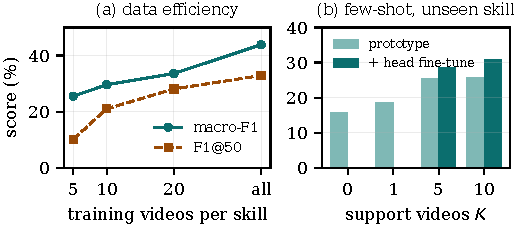
\includegraphics[width=\columnwidth]{figures/data_efficiency.pdf}
\caption{(a) Test scores of CLIP + MS-TCN versus training videos per skill. (b) Few-shot macro-F1 on the held-out
CookOmelet skill: prototypes from $K$ support videos and head-only fine-tuning.}
\label{fig:eff}
\end{figure}

\textbf{Generalisation to new videos.} On ten further COIN test videos run on a laptop CPU (four library and six demo
candidates), the deployed model obtains a mean macro-F1 of 41.0 (range 25.0--68.8), in line with the test-set average,
and needs 1.11\,s of CPU time per second of video.

\subsection{Case study and grounding}
Fig.~\ref{fig:cpr} shows the 120\,s CPR video used in the provider comparison. The recogniser finds five steps that
match the ground-truth order exactly (edit score 100) with macro-F1 79.3, F1@50 80.0 and boundary F1 75.0. All Hindi
and Kannada clips fit their steps: only one clip needed a speed-up (1.036$\times$) and no narration overflowed into the
next step.

\begin{figure}[t]
\centering
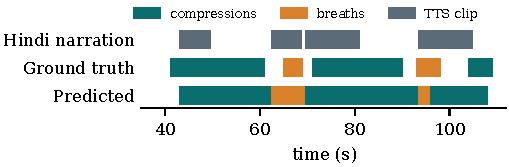
\includegraphics[width=\columnwidth]{figures/cpr_timeline.pdf}
\caption{CPR test video: COIN ground truth, predicted steps and the placed Hindi narration clips.}
\label{fig:cpr}
\end{figure}

To measure grounding, we compared the content words of the generated narration with the transcript and the step
labels. Six word types are not found in either source. Four are paraphrases (\emph{pausing, rescue, resume,
immediately}); two (\emph{carotid artery}) add an anatomical detail that the instructor never mentions. The detail is
correct, but it shows why the system makes trainer review mandatory and forbids added facts in the prompt.

\subsection{Speech stack: API versus open models}
Fig.~\ref{fig:lat} and Table~\ref{tab:stack} compare the two speech stacks on the CPR video. The two recognisers agree
closely (4.5\% word error rate of Whisper-small against Sarvam); Whisper additionally emitted a spurious ``Music'' token.
IndicTrans2 and Sarvam translations agree with a chrF of 75.8 for Hindi and 69.8 for Kannada, and reading both shows
mostly lexical differences, for example native versus borrowed medical terms. The large gap is in synthesis: Indic
Parler-TTS needs 3.34\,s per second of audio on a T4, while Sarvam's Bulbul returns audio in 0.52\,s per second. The
AI4Bharat IndicConformer recogniser could not be loaded in this run because ONNX Runtime rejected its cached external
weight files.

\begin{figure}[t]
\centering
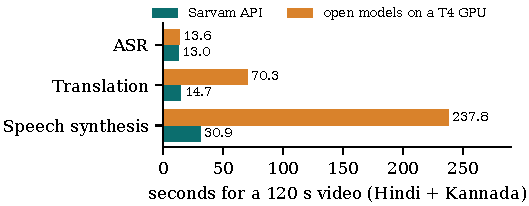
\includegraphics[width=\columnwidth]{figures/latency.pdf}
\caption{Stage latency for the 120\,s CPR video (two target languages).}
\label{fig:lat}
\end{figure}

\begin{table}[t]
\centering
\caption{Speech stacks on the CPR test video (Kaggle T4). RTF: synthesis time / audio duration.}
\label{tab:stack}
\setlength{\tabcolsep}{3pt}
\begin{tabular}{@{}llcl@{}}
\toprule
Stage & System & Time (s) & Quality / cost \\
\midrule
\multirow{2}{*}{ASR} & Whisper-small & 13.6 (+47 load) & WER 4.5 vs.\ Sarvam; free \\
 & Sarvam & 13.0 & \rup0.49/min \\
\midrule
\multirow{2}{*}{MT} & IndicTrans2-200M & 70.3 & chrF agreement 75.8 hi / \\
 & Sarvam Translate & 14.7 & 69.8 kn; \rup2 per 1k chars \\
\midrule
\multirow{2}{*}{TTS} & Indic Parler-TTS & 237.8 & RTF 3.34; free \\
 & Sarvam Bulbul v3 & 30.9 & RTF 0.52; \rup3 per 1k chars \\
\bottomrule
\end{tabular}
\end{table}

\subsection{End-to-end cost and latency}
Table~\ref{tab:cost} reports the full pipeline on 30 unseen test videos with Sarvam for all speech stages. Dubbing one
video into two languages costs \rup4.07 on average (\rup2.53 per minute of source video) and takes 4.6 minutes; step recognition on the CPU accounts for about 1.8 of these minutes
(1.11\,s per second of video). The whole library cost \rup121.98, or \rup127.33 including
retried attempts. With the open stack on a free T4, the provider cost drops to zero, but the 120\,s CPR video took about
nine minutes end to end, dominated by speech synthesis (238\,s) and LLM retries on an overloaded endpoint (155\,s);
the open stack suits bulk processing and the API stack interactive use. The primary LLM was frequently overloaded during
the run; the fallback chain produced valid step text for all 30 videos (29 from Groq, one from a second Gemini model) and
the template fallback was never needed.

\begin{table}[t]
\centering
\caption{End-to-end results for 30 unseen COIN test videos (Sarvam stack, Hindi + Kannada).}
\label{tab:cost}
\setlength{\tabcolsep}{3.5pt}
\begin{tabular}{@{}lccccc@{}}
\toprule
Domain & Videos & Length (s) & Steps & \rup/video & Min/video \\
\midrule
First aid & 5 & 86 & 4.0 & 4.13 & 4.6 \\
Phone repair & 5 & 89 & 4.8 & 4.43 & 4.5 \\
Car care & 5 & 90 & 3.6 & 4.34 & 5.4 \\
Cooking & 15 & 104 & 3.8 & 3.83 & 4.3 \\
\midrule
All & 30 & 96 & 3.9 & 4.07 & 4.6 \\
\bottomrule
\end{tabular}
\end{table}

\subsection{Implementation}
The system is deployed as a web application with three roles. Trainers upload, review and publish; learners watch with
per-language audio and captions, take quizzes and report problems at a timestamp; annotators correct step boundaries. A
FastAPI service enqueues jobs on Redis; the same worker code runs on a CPU server and in a GPU notebook for the open
models. Postgres with row-level security and object storage hold videos and outputs. Each job records its stages,
providers and estimated cost. Out-of-credit responses (HTTP 402) are not retried but trigger a fallback to the next
provider, while rate limits (HTTP 429) are retried with back-off. User API keys are stored encrypted.

\textbf{Limitations.} COIN annotations are coarse and the test sets are small (14--23 videos per skill). We did not run a
listening test, so voice quality is compared only through latency and agreement measures. Grounding was checked
automatically on one video and needs a larger human evaluation.

\section{Conclusion and Future Work}
KaushalDub shows that visual step segmentation is a practical backbone for dubbing procedural videos into Indian
languages. Among five architectures, CLIP features with an MS-TCN and cosine heads offer the best balance of accuracy,
calibration, size and training cost, and the same design enables few-shot skills and an annotator-driven correction
memory. A complete Hindi and Kannada dub costs about four rupees and five minutes per video with a commercial API, or
nothing on a free GPU at lower speed. Future work includes a listening test with learners, full-speech dubbing with
voice separation, more skills from crowd-sourced corrections, and evaluating attention-based temporal models.

\begin{thebibliography}{99}
\bibitem{tang2019coin} Y. Tang, D. Ding, Y. Rao, Y. Zheng, D. Zhang, L. Zhao, J. Lu, and J. Zhou, ``COIN: A large-scale
dataset for comprehensive instructional video analysis,'' in \emph{Proc. IEEE/CVF CVPR}, 2019, pp. 1207--1216.
\bibitem{farha2019mstcn} Y. A. Farha and J. Gall, ``MS-TCN: Multi-stage temporal convolutional network for action
segmentation,'' in \emph{Proc. IEEE/CVF CVPR}, 2019, pp. 3575--3584.
\bibitem{yi2021asformer} F. Yi, H. Wen, and T. Jiang, ``ASFormer: Transformer for action segmentation,'' in
\emph{Proc. BMVC}, 2021.
\bibitem{lea2017tcn} C. Lea, M. D. Flynn, R. Vidal, A. Reiter, and G. D. Hager, ``Temporal convolutional networks for
action segmentation and detection,'' in \emph{Proc. IEEE CVPR}, 2017, pp. 156--165.
\bibitem{zhukov2019crosstask} D. Zhukov, J.-B. Alayrac, R. G. Cinbis, D. Fouhey, I. Laptev, and J. Sivic, ``Cross-task
weakly supervised learning from instructional videos,'' in \emph{Proc. IEEE/CVF CVPR}, 2019, pp. 3537--3545.
\bibitem{miech2019howto100m} A. Miech, D. Zhukov, J.-B. Alayrac, M. Tapaswi, I. Laptev, and J. Sivic, ``HowTo100M:
Learning a text-video embedding by watching hundred million narrated video clips,'' in \emph{Proc. IEEE/CVF ICCV}, 2019.
\bibitem{radford2021clip} A. Radford \emph{et al.}, ``Learning transferable visual models from natural language
supervision,'' in \emph{Proc. ICML}, 2021, pp. 8748--8763.
\bibitem{ni2022xclip} B. Ni \emph{et al.}, ``Expanding language-image pretrained models for general video
recognition,'' in \emph{Proc. ECCV}, 2022, pp. 1--18.
\bibitem{he2016resnet} K. He, X. Zhang, S. Ren, and J. Sun, ``Deep residual learning for image recognition,'' in
\emph{Proc. IEEE CVPR}, 2016, pp. 770--778.
\bibitem{hochreiter1997lstm} S. Hochreiter and J. Schmidhuber, ``Long short-term memory,'' \emph{Neural Computation},
vol. 9, no. 8, pp. 1735--1780, 1997.
\bibitem{radford2023whisper} A. Radford, J. W. Kim, T. Xu, G. Brockman, C. McLeavey, and I. Sutskever, ``Robust speech
recognition via large-scale weak supervision,'' in \emph{Proc. ICML}, 2023, pp. 28492--28518.
\bibitem{gala2023indictrans2} J. Gala \emph{et al.}, ``IndicTrans2: Towards high-quality and accessible machine
translation models for all 22 scheduled Indian languages,'' \emph{Trans. Mach. Learn. Res.}, 2023.
\bibitem{bhogale2023vistaar} K. S. Bhogale \emph{et al.}, ``Vistaar: Diverse benchmarks and training sets for Indian
language ASR,'' in \emph{Proc. Interspeech}, 2023.
\bibitem{lyth2024parler} D. Lyth and S. King, ``Natural language guidance of high-fidelity text-to-speech with
synthetic annotations,'' arXiv:2402.01912, 2024.
\bibitem{federico2020dubbing} M. Federico \emph{et al.}, ``From speech-to-speech translation to automatic dubbing,'' in
\emph{Proc. IWSLT}, 2020, pp. 257--264.
\bibitem{oktem2019prosodic} A. \"Oktem, M. Farr\'us, and A. Bonafonte, ``Prosodic phrase alignment for machine
dubbing,'' in \emph{Proc. Interspeech}, 2019, pp. 4215--4219.
\bibitem{guo2017calibration} C. Guo, G. Pleiss, Y. Sun, and K. Q. Weinberger, ``On calibration of modern neural
networks,'' in \emph{Proc. ICML}, 2017, pp. 1321--1330.
\bibitem{settles2009active} B. Settles, ``Active learning literature survey,'' Univ. Wisconsin--Madison, Comput. Sci.
Tech. Rep. 1648, 2009.
\bibitem{gemini2023} Gemini Team, Google, ``Gemini: A family of highly capable multimodal models,'' arXiv:2312.11805,
2023.
\bibitem{sarvam2026pricing} Sarvam AI, ``API pricing.'' [Online]. Available: https://www.sarvam.ai/api-pricing
(accessed Nov. 7, 2026).
\end{thebibliography}

\end{document}
